\chapter{神经网络概述}
\label{chap:neural-network-overview}

先考虑一个朴素的垃圾邮件判别器。我们从每封邮件中统计两个数字：促销提示词出现的次数$x_1$、邮件里外部链接的数量$x_2$，再用线性分类器计算得分
\[
  s=w_1x_1+w_2x_2+b,
\]
得分超过阈值就判为垃圾邮件。这里真正从数据中学到的只有三个数：两个权重$w_1,w_2$和一个常数$b$（称为偏置，相当于把阈值折算进得分）。

这个模型可以学得不错，但它的能力上限在我们统计$x_1,x_2$的那一刻就已经决定了。假如垃圾邮件的关键特征不是“促销词多不多”，而是“促销词和链接紧挨着出现”这样的搭配关系，仅凭两个各自独立的计数无法把它表达出来：两封促销词数和链接数相同的邮件，搭配方式可能完全不同，得分却必然一样。要利用搭配，就得有人先想到去统计“促销词旁边是否有链接”这个新数字。换句话说，\emph{统计什么特征}仍然依赖人的判断，学习算法只能在人给定的特征上调整系数。

如果特征搭配非常多——词语搭配、图像里边缘的组合、语音里相邻音素的关系——靠人工逐一列举就不现实了。能否让模型自己去发现“哪些组合有用”？这正是\term{人工神经网络}（artificial neural network, ANN）试图回答的问题。它由大量相互连接的简单计算单元组成，每个单元把收到的数值组合起来再作一次变换，而决定这些连接强弱的参数（包括连接权重和偏置）全部通过数据学习。与线性分类器只学“输出层系数”不同，神经网络把\emph{输入特征如何被改写}也纳入了学习范围：先根据任务要求调整输入的内部表示，再用这个表示完成预测。

本章面向初次接触神经网络的读者，回答四个问题：第一，“可学习的表示”到底改变了什么，为什么它比直接在原始特征上分类更强（\ref{sec:neural-learned-representations}节）；第二，这套受生物启发的术语——神经元、连接、学习——与真实神经系统有几分相似（\ref{sec:neural-biological-inspiration}节）；第三，面对卷积、循环、注意力等大量名字，应该按什么标准给网络分类（\ref{sec:neural-network-types}节）；第四，这些方法是在解决什么问题的过程中先后出现的（\ref{sec:neural-history}节）。阅读本章只需要线性代数中的向量与矩阵运算、微积分中的偏导数概念，以及前几卷介绍过的基本学习流程：用损失函数衡量预测与标签的差距，再用梯度下降调整参数。具体网络的结构细节和训练推导留待后续各章。

\section{从人工特征到可学习的表示}
\label{sec:neural-learned-representations}

我们先通过一个具体网络看“学习特征”是如何发生的。图~\ref{fig:neural-minimal-mlp}是一个用于前述邮件分类任务的小型网络：两个输入$x_1,x_2$在左侧，中间有三个单元$h_1,h_2,h_3$，右侧是一个输出单元。

\begin{figure}[htbp]
  \centering
  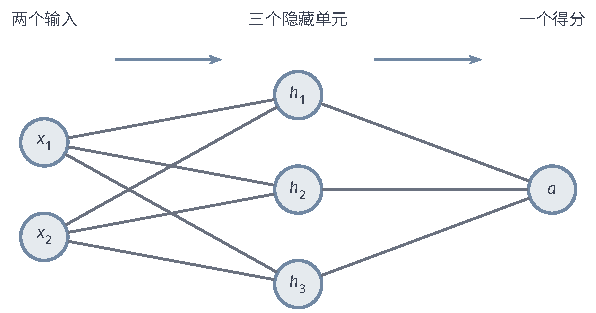
\includegraphics[width=100.993mm]{figures/05-neural-network-models/00-shared/tikz/neural-minimal-mlp/figure.pdf}
  \caption{一个$2$-$3$-$1$多层感知机：两个输入经过三个隐藏单元，得到一个分类得分。连线表示带权连接，箭头表示计算方向；隐藏单元作非线性变换，偏置未画出。}
  \label{fig:neural-minimal-mlp}
\end{figure}
\FloatBarrier

图中的每条连线都带有一个权重。以第一个中间单元为例，它先对两个输入作加权求和并加上自己的偏置，再把总和送入一个非线性函数（下一小节会说明为什么这一步不可或缺）：
\[
  a_1=w_{11}x_1+w_{21}x_2+b_1,\qquad h_1=\rho(a_1).
\]
另外两个单元$h_2,h_3$的算法完全相同，只是权重和偏置不同。于是，从同样两个计数出发，网络得到了三个新数字。输出单元再把这三个数字加权组合成分类得分：
\[
  s=v_1h_1+v_2h_2+v_3h_3+c.
\]
为获得具体感受，可以代入一组教学数值。假设$h_1$的权重为$w_{11}=1,w_{21}=-1$，偏置$b_1=0$，且$\rho(a)=\max\{0,a\}$（负的总和被截为零）。那么$h_1=\max\{0,x_1-x_2\}$只在“促销词数明显多于链接数”时才取非零值——这已经是一种关于两个特征\emph{搭配关系}的描述，尽管这里的权重是我们手填的。真实训练中，$w$、$b$、$v$、$c$都由梯度下降根据分类错误自动调整：如果某个中间单元的输出有助于降低错误，与它相连的权重就会朝相应方向改变，直到它稳定地检测某种对任务有用的模式。

这三个中间单元的数值不来自外界输入，也不直接作为最终答案，它们是网络内部的中间产物，因此称为\term{隐藏层}（hidden layer）。“隐藏”不是说它们不可观测，而是说它们的取值不构成训练数据：我们从不提供“$h_1$应该等于多少”的标签，只提供最终的垃圾邮件标签，让学习算法自己决定每个隐藏单元该检测什么。图中相邻两层之间两两相连、信息逐层向前流动，这种结构称为\term{多层感知机}（multilayer perceptron, MLP）。名字里的“感知机”源自早期的一种单层模型（见\ref{sec:neural-history-threshold}节），今天它已泛指这种由全连接层堆叠而成的网络。

需要强调的是，学习隐藏层不等于无中生有。网络只能重组输入中已经保留的信息：如果两封邮件被编码成完全相同的$(x_1,x_2)$，那么无论隐藏层多复杂，算出的$h_1,h_2,h_3$都相同，网络无法恢复编码阶段已经丢失的词序或上下文。因此，“让网络学习特征”并不取消输入编码的责任，而是把“该统计哪些组合”这一层决策，从人工提前固定改为在任务信号引导下从数据中形成。下一小节先从函数复合的角度说明这种改写为什么能增强能力。

\subsection{特征变换与函数复合}
\label{sec:neural-feature-composition}

表示变换的作用，是把输入改写到一个对任务更友好的坐标系中。仍以分类为例：线性分类器只能在输入空间中画一条直线（或一个超平面）作为两类的分界。若两类点在原坐标中犬牙交错，任何直线都分不开它们；但如果先把点映到一组新坐标，使正类聚在一起、负类聚在一起，在新坐标系中画一条直线就足够了。下面先给出形式化记号，再用一个最小例子展示这次“改写”的效果。

将可学习的表示变换记为$\bm{r}_{\bm{\theta}}(\bm{x})$，它把原始输入$\bm{x}$映为一个表示向量；再把利用表示产生预测的输出映射记为$g_{\bm{\psi}}$。整个网络就是两个函数的复合：
\begin{equation}
  f_{\bm{\theta},\bm{\psi}}(\bm{x})
  =g_{\bm{\psi}}\!\left(\bm{r}_{\bm{\theta}}(\bm{x})\right),
  \label{eq:neural-representation-readout}
\end{equation}
其中$\bm{\theta}$和$\bm{\psi}$分别是表示部分与输出部分的参数。在线性分类器中，表示是固定的（直接用$\bm{x}$），只有$g$的参数在学；神经网络中$\bm{\theta}$也在学，即“用什么坐标描述样本”本身成为学习对象。这种从数据中学习供后续任务使用的信息形式的做法，称为\term{表示学习}（representation learning）。

表示部分还可以由多层变换复合而成：上一层的输出作为下一层的输入，每层先作加权求和并加偏置，再通过一个\term{激活函数}（activation function）——一个逐元素作用的固定非线性函数，决定单元在多大输入下以多强的程度响应——作非线性变换。

\paragraph{为什么非线性不可省略。}
这是初学时最需要想清楚的一点。假设网络完全不使用非线性激活，两层的计算分别是
\[
  \bm{h}=\bm{W}_1\bm{x}+\bm{b}_1,\qquad
  \bm{s}=\bm{W}_2\bm{h}+\bm{b}_2.
\]
把第一式代入第二式：
\[
  \bm{s}=\bm{W}_2(\bm{W}_1\bm{x}+\bm{b}_1)+\bm{b}_2
       =(\bm{W}_2\bm{W}_1)\bm{x}+(\bm{W}_2\bm{b}_1+\bm{b}_2).
\]
令$\bm{W}=\bm{W}_2\bm{W}_1$、$\bm{b}=\bm{W}_2\bm{b}_1+\bm{b}_2$，两层网络就退化成$\bm{s}=\bm{W}\bm{x}+\bm{b}$——仍是输入的一个线性函数，与只有一层完全等价。重复同样的代入可知，任意多层线性变换的复合还是线性变换。这意味着：如果没有非线性，无论叠多少层，网络能画的分类边界仍然是一个超平面，深度不带来任何新能力。非线性激活的作用，正是打破这种可合并性，使每一层都可能把坐标系“弯折”到线性模型无法达到的形状。

\begin{example}[异或的表示变换]
  \label{ex:neural-xor-representation}
  \term{异或}（exclusive OR, XOR）要求：两个二值输入$x_1,x_2$不同时输出$1$，相同时输出$0$，即四个样本为
  \[
    (0,0)\mapsto 0,\quad (1,1)\mapsto 0,\quad (0,1)\mapsto 1,\quad (1,0)\mapsto 1.
  \]
  图~\ref{fig:neural-xor-representation}左侧可以看到，两个负例（圆点）处在对角线上，两个正例（方点）处在另一条对角线上，任何一条直线都无法把两类分开——这正是纯线性模型的失败情形。

  取\term{整流线性单元}（rectified linear unit, ReLU）激活函数$\rho(a)=\max\{0,a\}$，它把负值置零、正值原样保留。构造两个隐藏单元
  \begin{equation}
    h_1=\rho(x_1-x_2),\qquad h_2=\rho(x_2-x_1).
    \label{eq:neural-xor-hidden}
  \end{equation}
  逐个样本代入：
  \begin{equation*}
    \begin{array}{c|cc|c}
      (x_1,x_2) & h_1=\rho(x_1-x_2) & h_2=\rho(x_2-x_1) & \text{标签} \\ \hline
      (0,0) & 0 & 0 & 0 \\
      (1,1) & 0 & 0 & 0 \\
      (0,1) & 0 & 1 & 1 \\
      (1,0) & 1 & 0 & 1
    \end{array}
  \end{equation*}
  两个输入相同时，$(h_1,h_2)$都是$(0,0)$；输入不同时，其中一个坐标为$1$。在新坐标系中，两个负例重合于原点，两个正例落在坐标轴上，用一条直线$h_1+h_2=1/2$（图中虚线）就把两类分开了，输出端只需判断$h_1+h_2>1/2$。图~\ref{fig:neural-xor-representation}右侧画出了这次变换的结果。

  这个例子说明的是隐藏表示\emph{能够}完成什么：一次坐标变换把线性不可分的问题变成线性可分。但式中的权重是手工构造的，它并不证明训练算法在真实问题上必然能找到这样的参数——“能表达”和“能学到”是两件不同的事。
\end{example}

\begin{figure}[htbp]
  \centering
  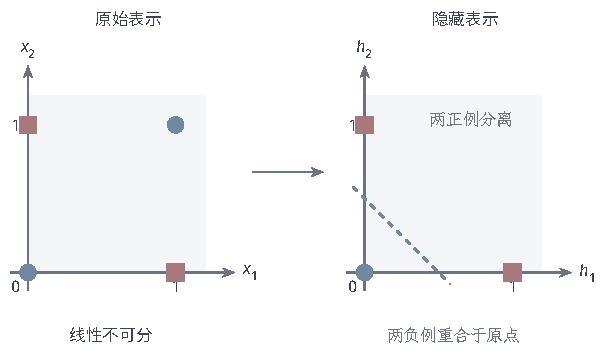
\includegraphics[width=102.902mm]{figures/05-neural-network-models/00-shared/tikz/neural-xor-representation/figure.pdf}
  \caption{异或任务的表示变换。圆点为负例，方点为正例。左侧无法用一条直线分开；按式\eqref{eq:neural-xor-hidden}变换后，右侧两个负例重合，虚线$h_1+h_2=1/2$将两类分开。坐标和变换均为教学构造。}
  \label{fig:neural-xor-representation}
\end{figure}

实际训练中，没有人手工给出隐藏层的目标值。学习算法先做一次前向计算得到预测，再用损失函数衡量预测与标签的差距，然后通过链式求导同时计算损失对$\bm{\theta}$和$\bm{\psi}$的梯度，一次性更新所有参数。这样，表示层的调整方向完全由“能否降低最终任务的损失”决定，无需为每个隐藏单元预先指定含义，这种训练方式称为\term{端到端学习}（end-to-end learning）——从原始输入到最终输出的整条映射作为一个整体接受同一个任务信号的训练。

由此必须区分三个常被混为一谈的问题。其一，\term{表示能力}（网络能不能表达完成任务所需的函数）：异或例子中的网络具备这种能力，但这只说明存在一组参数可行。其二，\term{优化}（训练算法能不能找到这组合适参数）：目标函数关于参数通常是非凸的，梯度下降可能停在较差的解。其三，\term{泛化}（学到的函数在未见样本上是否仍然有效）：在训练样本上把损失降到零，只说明记住了这些样本，不代表新样本也能正确处理。后续章节会反复回到这三个问题；本章只要求读者记住，肯定其中一个并不自动肯定另外两个。

\subsection{分布式表示与层次表示}
\label{sec:neural-distributed-hierarchical}

知道隐藏层能改造坐标后，进一步要问：多个单元、多层单元分别是怎样组织信息的？这两个问题对应两种相互正交的设计，理解它们有助于读懂后续所有架构图。

\term{分布式表示}（distributed representation）关注\emph{同一层内部}如何组织信息：一个对象由多个单元的活动共同表示，同一个单元又可以参与多个对象的表示。设想用三个单元分别编码“是否偏红”“是否圆形”“是否较大”，那么“红苹果”“红皮球”“青苹果”由这三个单元的不同活动组合区分，而不需要为每种物体单独分配一个单元。这种组织的好处是组合性：$k$个取值连续的单元可以形成大量不同的活动模式，识别一个新组合时也可能复用已有的各属性检测。需要澄清的是，实际网络中的隐藏坐标通常是连续数值，也未必分别对应某个可命名的属性；这里的“分布式”指信息分散承载在多个单元的联合活动中，与“多台计算机分布计算”无关\scite{goodfellow2016}

\term{层次表示}（hierarchical representation）关注\emph{不同层之间}如何组合信息：后一层把前一层的表示当作输入，在更高的抽象级别上构造新特征。以图像识别为例，第一层隐藏单元可能只响应局部的明暗突变（边缘小段）；第二层把相邻、方向一致的响应组合起来，得到对线条或拐角的检测；再往后组合成简单形状，直至与物体部件、整体物体对应的表示。后一层之所以能表示更复杂的东西，正是因为它建立在前一层已经提炼过的信息上。需要说明，层次表示描述的是这种逐层组合的关系，并不要求每一层都对应一个人类可命名的概念，也不保证层数越多表示就越有用——过深的网络在数据或训练方法不足时可能更难优化。

两种方式同时存在于一个网络中：每层内部用多个单元共同表示输入（分布式），层与层之间逐级组合这些活动（层次化），最终完成任务。图~\ref{fig:neural-representation-path}把这条路径画在一起：实线是预测时输入经各层变换得到输出的方向，虚线是训练时任务损失反向指导每一层参数调整的方向。

\begin{figure}[htbp]
  \centering
  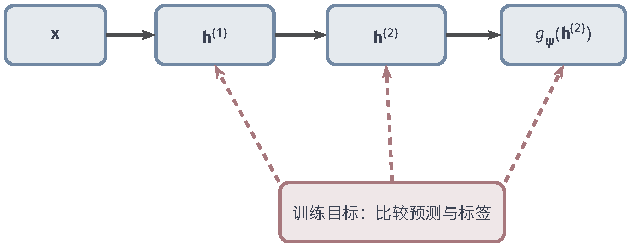
\includegraphics[width=106.793mm]{figures/05-neural-network-models/00-shared/tikz/neural-representation-path/figure.pdf}
  \caption{表示学习的计算路径。实线表示输入经各层变换得到预测，虚线表示训练目标指导表示层与输出层的参数调整。隐藏坐标无需具有预先指定的语义。}
  \label{fig:neural-representation-path}
\end{figure}

\subsection{结构带来的归纳偏置}
\label{sec:neural-structural-bias}

理论上，一个足够宽的多层感知机可以读取所有输入并让它们任意交互。那么为什么还需要卷积网络、循环网络这些专门结构？原因在于数据量和计算量都有限：若对所有任务都用全连接的通用网络，模型要么需要多得多的样本才能确定海量参数，要么在有限样本上学出不稳定的规律。如果我们事先知道数据中存在某些结构，把这种知识“写进”网络的连接方式，学习就会容易得多。

结构预先规定了两件事：哪些信息之间可以发生相互作用，哪些计算可以在不同位置或不同时刻重复使用。这些规定体现了模型对数据规律的假设。在有限样本下，任何能引导学习朝某类解收敛、并帮助模型推广到新样本的限制或偏好，统称为\term{归纳偏置}（inductive bias）。“偏置”在这里不是贬义的成见，而是学习能够发生的前提——没有任何偏好的模型面对有限数据无从选择。归纳偏置除了来自网络结构，也可以来自损失函数的形式或学习算法本身，这里主要讨论结构带来的偏置。

例如，图像数据有两条常见规律：有意义的模式通常由空间上相邻的像素构成，而同一种模式（如一条竖直边缘）可能出现在画面任何位置。针对前一条，\term{局部连接}（local connectivity）让每个单元只读取输入的一小块邻域，而不与整张图相连，强迫单元专注于局部模式；针对后一条，\term{参数共享}（parameter sharing）让同一组权重在图像的不同位置复用，使“在左上角学到的边缘检测”无需重新学习就能用于右下角。再如语言和语音这样的序列，当前判断往往依赖此前的内容，网络可以用一个\term{隐状态}（hidden state）——一个随处理过程不断更新的内部向量，可理解为网络递给下一步自己的“摘要便签”——保存由历史输入计算得到的信息，供后续时刻使用。

这些设计有助于利用数据中的规律、减少需要确定的参数量，但任何偏置都是双刃剑：它同时限制了模型能够表达的函数族。若任务本身不符合假设（例如强迫只看局部的网络判断需要全图布局的关系），偏置反而会妨碍学习。因此某种架构表示能力强，不等于它必然容易训练或一定泛化得好，结构是否合适需要结合任务判断。关于表示能力的形式化结论，可参考\BookChapterRef{chap:deep-learning-theory}{卷3《基础、理论与可信性》的“深度学习的可学习性”章}。

\section{生物神经网络}
\label{sec:neural-biological-inspiration}

神经网络的名字和术语大量借用自神经科学：“神经元”“连接”“学习”“激活”。这些类比是历史形成的——早期研究者确实希望用电路模拟智能——但今天工程上有效的神经网络，其数学与真实神经系统的差距已经很大。本节按三条线索梳理这种关系：单个神经细胞如何通信（\ref{sec:neural-biological-unit}节）、大量细胞如何组成处理系统（\ref{sec:neural-biological-system}节）、经验如何改变连接（\ref{sec:neural-biological-learning}节），最后在\ref{sec:neural-biological-comparison}节对照人工单元与人工网络，说明哪些相似是实质性的功能抽象，哪些只是名词借用。

\subsection{神经元}
\label{sec:neural-biological-unit}

生物\term{神经元}（neuron）是神经系统中接收、处理和传递信号的细胞。一个典型神经元分为三部分：大量树突负责从其他细胞接收信号，胞体进行整合，一根轴突把信号传给其他细胞。输入信号会改变细胞膜内外带电离子的浓度差，即\term{膜电位}（membrane potential）。单个输入通常很微弱，胞体把来自许多连接、在不同时刻到达的影响累加起来：当膜电位升高到某个阈值附近，细胞就触发一次\term{动作电位}（action potential）——一个持续约一毫秒、沿轴突主动传导的短暂电脉冲，也称“发放一次”；脉冲过后膜电位恢复，细胞经过短暂不应期才能再次发放。轴突末梢与下一个细胞的树突或胞体之间有微小间隙，这个传递影响的连接部位称为\term{突触}（synapse）。图~\ref{fig:neural-biological-neuron}展示一个细胞通过轴突分支向另外两个细胞传递信号的结构\scite{purves2001}

\begin{figure*}[!t]
  \centering
  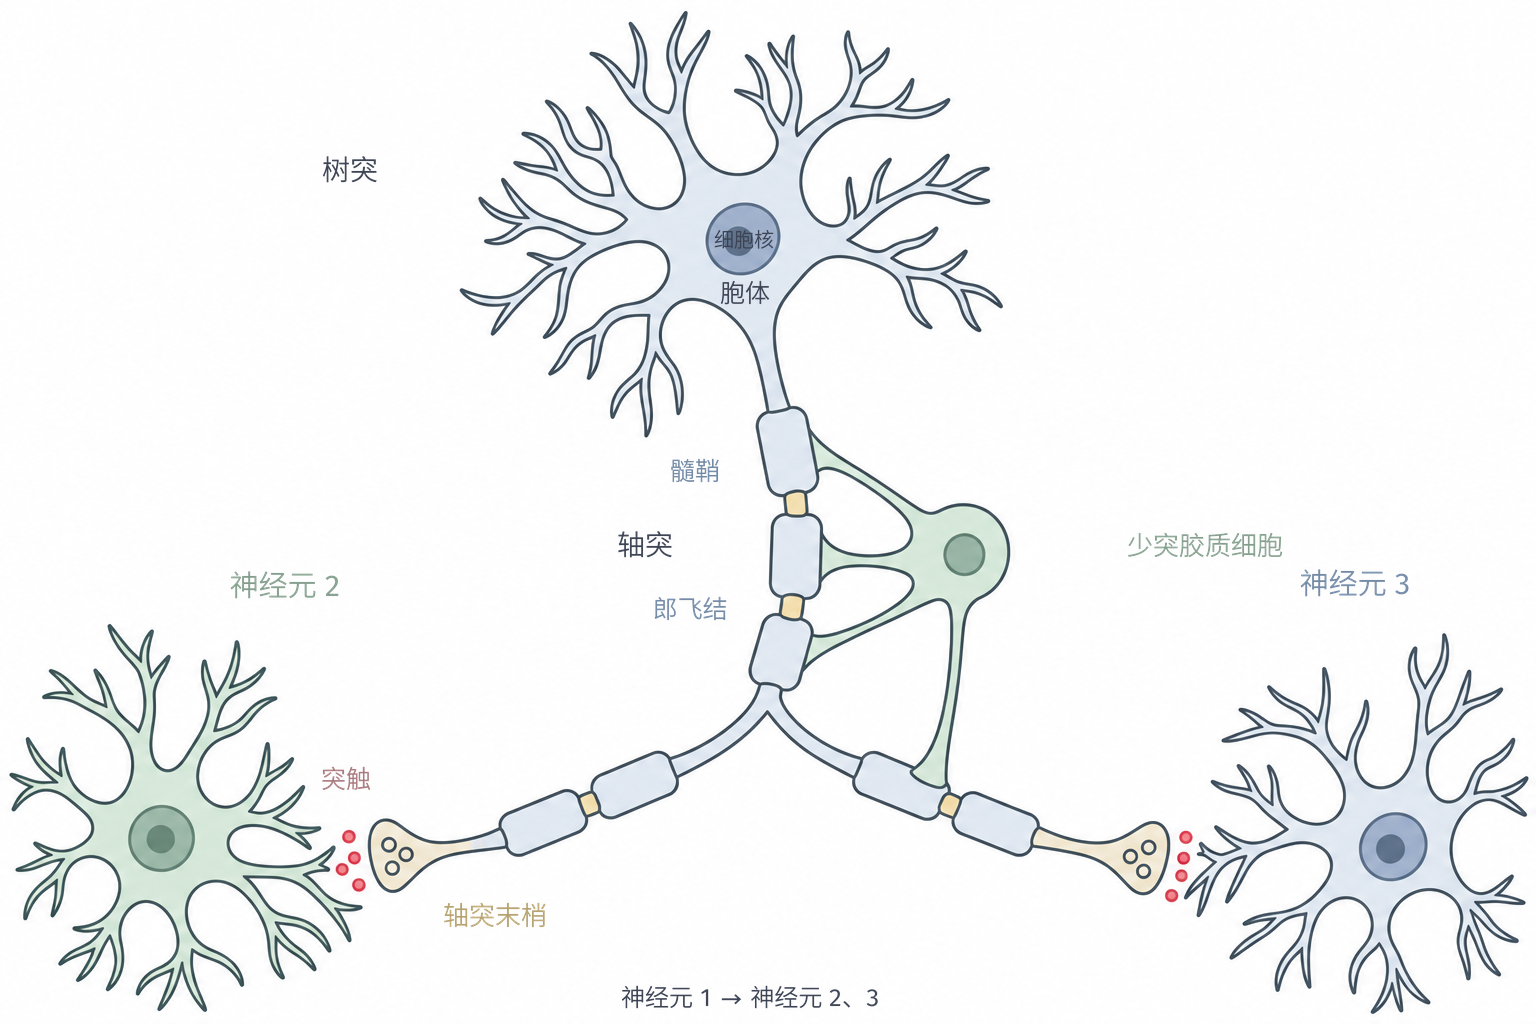
\includegraphics[width=130.048mm]{figures/05-neural-network-models/00-shared/generated/neural-biological-neuron/figure.png}
  \caption{三个神经元通过突触相连。神经元1的轴突分支分别联系神经元2和3，表示一个细胞可以影响多个细胞。图示一种有髓鞘的多极神经元形态，髓鞘段之间的间隙为郎飞结；各部分不按比例，真实神经元形态多样，并非所有轴突都有髓鞘。}
  \label{fig:neural-biological-neuron}
\end{figure*}

在最常见的化学突触中，脉冲到达轴突末梢会促使末梢释放神经递质，递质扩散过间隙、改变接收细胞膜上的离子通道，从而升高或降低它的膜电位。因此一个突触的作用可能是\emph{兴奋性}的（促进接收细胞发放），也可能是\emph{抑制性}的（压低发放倾向），并不保证“来一个输入就产生一个脉冲”。是否发放取决于许多突触输入与细胞当前状态的共同整合：不仅输入的数量和强弱有关，到达的时间排布也有关——同样数量的脉冲，密集到达可能越过阈值，分散到达则可能在恢复中相互抵消。正因为真实细胞的响应同时依赖输入内容、时间和内部状态，它无法被“固定权重的静态加权和”完整描述；人工单元（见\ref{sec:neural-biological-comparison}节）保留的只是“多输入整合后决定输出”这一层抽象\scite{gerstner2014}

\FloatBarrier
\subsection{神经系统}
\label{sec:neural-biological-system}

单个细胞的发放不足以解释看、记、动作这些整体功能。神经元先在局部组成回路，回路之间再通过有组织的长距离纤维束连接，形成分工协作的脑区系统。一个脑区的活动取决于它接收的输入、区内细胞的连接方式、当前的兴奋或抑制状态，以及从高级区域返回的反馈连接；因此神经元的数量本身不能直接换算成计算能力，连接的组织方式同样关键\scite{purves2001}

以研究得最充分的视觉为例，图~\ref{fig:neural-visual-pathways}概括了一条主要通路：光线在视网膜被转换成神经信号，经丘脑的外侧膝状体（LGN）中继，到达大脑后部的初级视觉皮层（V1），再向更高皮层区域发散。之后大致形成两条分工不同的通路：\term{腹侧视觉通路}（ventral visual stream）向颞叶延伸，偏重处理颜色、形状和物体身份，常被称为内容通路what；\term{背侧视觉通路}（dorsal visual stream）向顶叶延伸，偏重运动、空间关系和视觉引导的动作，常被称为空间通路where。这种分工在日常动作中可以直接体会：看到桌上的杯子时，“认出它是杯子”（是什么）与“判断杯子的位置、控制手伸过去并张开合适的角度”（怎样抓）由不同但相互配合的信息支持。真实视觉系统还包含大量跨通路联系和从高级区域返回低级区域的反馈，并非一次从前往后的单向传递\scite{purves2001,goodale1992}

\begin{figure*}[!t]
  \centering
  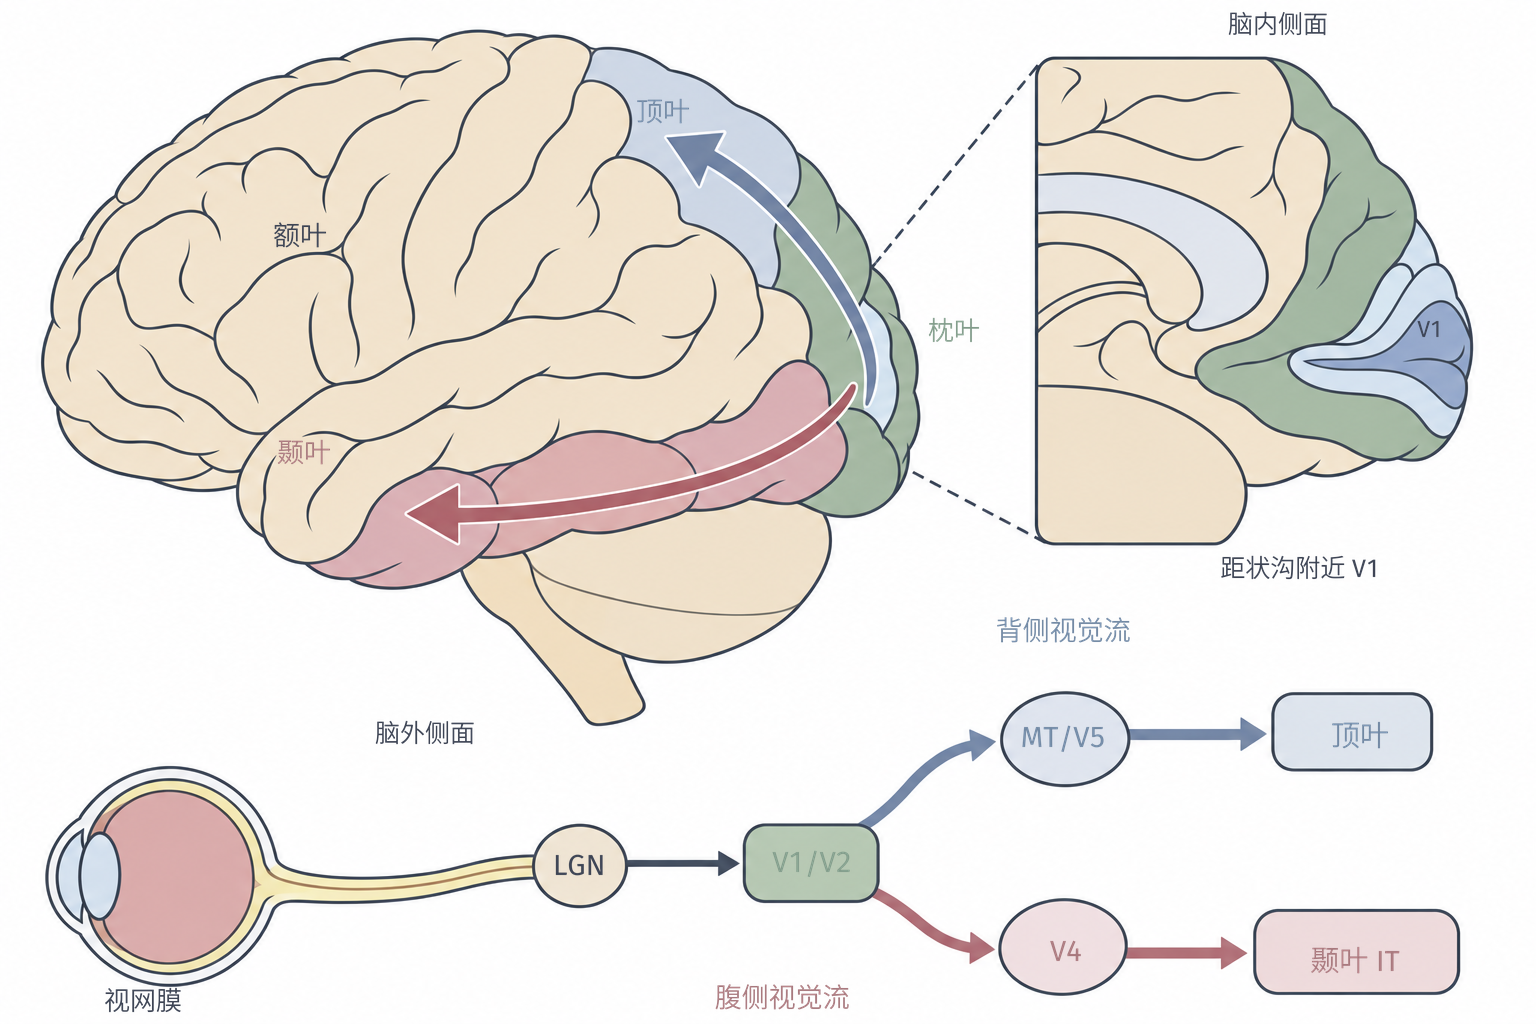
\includegraphics[width=130.048mm]{figures/05-neural-network-models/00-shared/generated/neural-visual-pathways/figure.png}
  \caption{人脑视觉区域与主要通路示意。视觉信号从视网膜经LGN进入V1/V2；蓝色分支经MT（V5）向顶叶传递空间与运动相关信息，红色分支经V4向下颞皮层IT传递物体相关信息。解剖图用于定位，箭头不表示精确边界、完整连接或唯一串行顺序，跨通路联系与反馈未画全。}
  \label{fig:neural-visual-pathways}
\end{figure*}

视觉系统中的一个关键概念是\term{感受野}（receptive field）：一个视觉神经元只受到视野中某一块有限区域内光刺激的影响，这块区域就是它的感受野；刺激落在感受野外，该神经元基本不响应。Hubel和Wiesel在20世纪60年代对猫视觉皮层的经典实验中发现，V1及附近区域的许多细胞并不对均匀光斑反应，而对特定取向、位置的局部光条有选择性，越往高级区域，细胞响应的模式越复杂、感受野越大。这种“先由局部检测、再逐层组合成复杂模式选择性”的组织方式，为人工网络的层次表示（见\ref{sec:neural-distributed-hierarchical}节）和卷积结构提供了生物学线索；但这只是原理层面的启发，不能据此认为某个人工计算层对应某个具体脑区\scite{hubel1962,purves2001}

\FloatBarrier
\subsection{生物学习}
\label{sec:neural-biological-learning}

前面描述的是神经系统在某一时刻如何响应。学习还要求回答另一个问题：经验怎样改变神经系统，使它今后的响应不同？

生物学习的物质基础发生在突触上。\term{突触可塑性}（synaptic plasticity）指突触传递效果能够随神经活动等因素持续改变——同一个突触，在特定的活动经历之后可能变强或变弱，而且这种改变可以保持一段时间。最有影响的一类概括称为\term{赫布学习}（Hebbian learning），常被通俗概括为“一起发放的细胞连得更紧”：如果突触前后两个神经元倾向于在相近时刻共同活动，这个突触的传递效果倾向于增强。它的直觉是把“反复同时出现”当作“两者相关、值得加强联系”的证据。后续研究进一步发现，活动的\emph{先后次序}也很关键：\term{脉冲时序依赖可塑性}（spike-timing-dependent plasticity, STDP）描述这样一类现象——突触前细胞略早于突触后细胞发放时，突触倾向于增强（前者像是后者发放的原因）；次序相反时则倾向于减弱。需要注意，STDP的具体方向和幅度受细胞类型、突触初始状态和实验方案影响，不存在所有突触统一遵守的一条规则\scite{bi1998,gerstner2018plasticity}

局部突触规则解释了连接如何随邻近活动改变，但学习的目的是改善整体行为，两者之间还隔着一个难题。练习伸手抓杯子时，如果这一次抓偏了，这个“偏差”是在动作末端才知道的；参与的神经元却遍布视觉、规划和运动控制的整条回路。究竟应该让回路中的哪些突触变强、哪些变弱，才能让下一次抓得更准？这就是\term{信用分配}（credit assignment）问题：整体结果应当如何追溯并影响内部各个环节。仅凭“两端一起发放”无法确定某条具体连接对这次行为偏差贡献了多少；大脑中可能由弥散的调节信号、反馈连接和多时间尺度的可塑性共同参与，但具体机制仍是开放的研究问题\scite{lillicrap2020}。这个问题在人工网络中同样存在，而工程上给出的答案（反向传播）将在\ref{sec:neural-biological-comparison}节末尾对照。

\subsection{与人工神经网络的对比}
\label{sec:neural-biological-comparison}

现在可以精确地说明人工单元从生物神经元那里保留了什么。对于输入向量$\bm{u}\in\mathbb{R}^{d}$，一种最常见的人工单元计算
\begin{equation}
  a=\sum_{j=1}^{d}w_j u_j+b,\qquad h=\sigma(a),
  \label{eq:neural-artificial-unit}
\end{equation}
如图~\ref{fig:neural-unit-abstraction}所示：各输入$u_j$乘以对应的权重$w_j$（对应突触可强可弱、可正可负的影响），求和后加偏置$b$（对应细胞固有的发放倾向），再经激活函数$\sigma$得到输出$h$（对应“整合后是否、以多强程度响应”）。这一公式保留的是功能层面的对应——接收多路输入、整合影响、产生输出；它没有复现脉冲的离散发放、抑制性与兴奋性递质的化学差异、膜电位的时间动态和各种不应期。生物神经元更像一个复杂的非线性时变系统，而式\eqref{eq:neural-artificial-unit}是一个静态的数学单元。

\begin{figure}[!t]
  \centering
  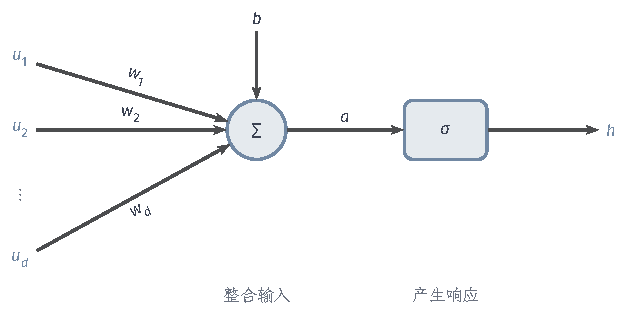
\includegraphics[width=106.161mm]{figures/05-neural-network-models/00-shared/tikz/neural-unit-abstraction/figure.pdf}
  \caption{人工单元先将各输入乘以权重，求和并加入偏置，再经激活函数产生输出。它保留接收、整合与输出的功能对应，数学运算不完整复现生物细胞。}
  \label{fig:neural-unit-abstraction}
\end{figure}

把多个单元连接起来后，比较的对象就从细胞上升为网络。图~\ref{fig:neural-biological-artificial-networks}将两者并置：真实神经回路中既有细胞类型的差异，也有局部小回路、跨区域长连接和大量反馈联系，信息往往在环路中反复流动；右侧的典型层状前馈网络则按人为规定的计算依赖，从输入经若干中间层一次性得到输出。当然，人工网络也可以加入环式连接（循环网络）和内部状态，因此不能笼统地断言“大脑有反馈而人工网络没有”——两者的比较必须落实到具体结构，更不能用节点数量简单类比。

\begin{figure*}[!t]
  \centering
  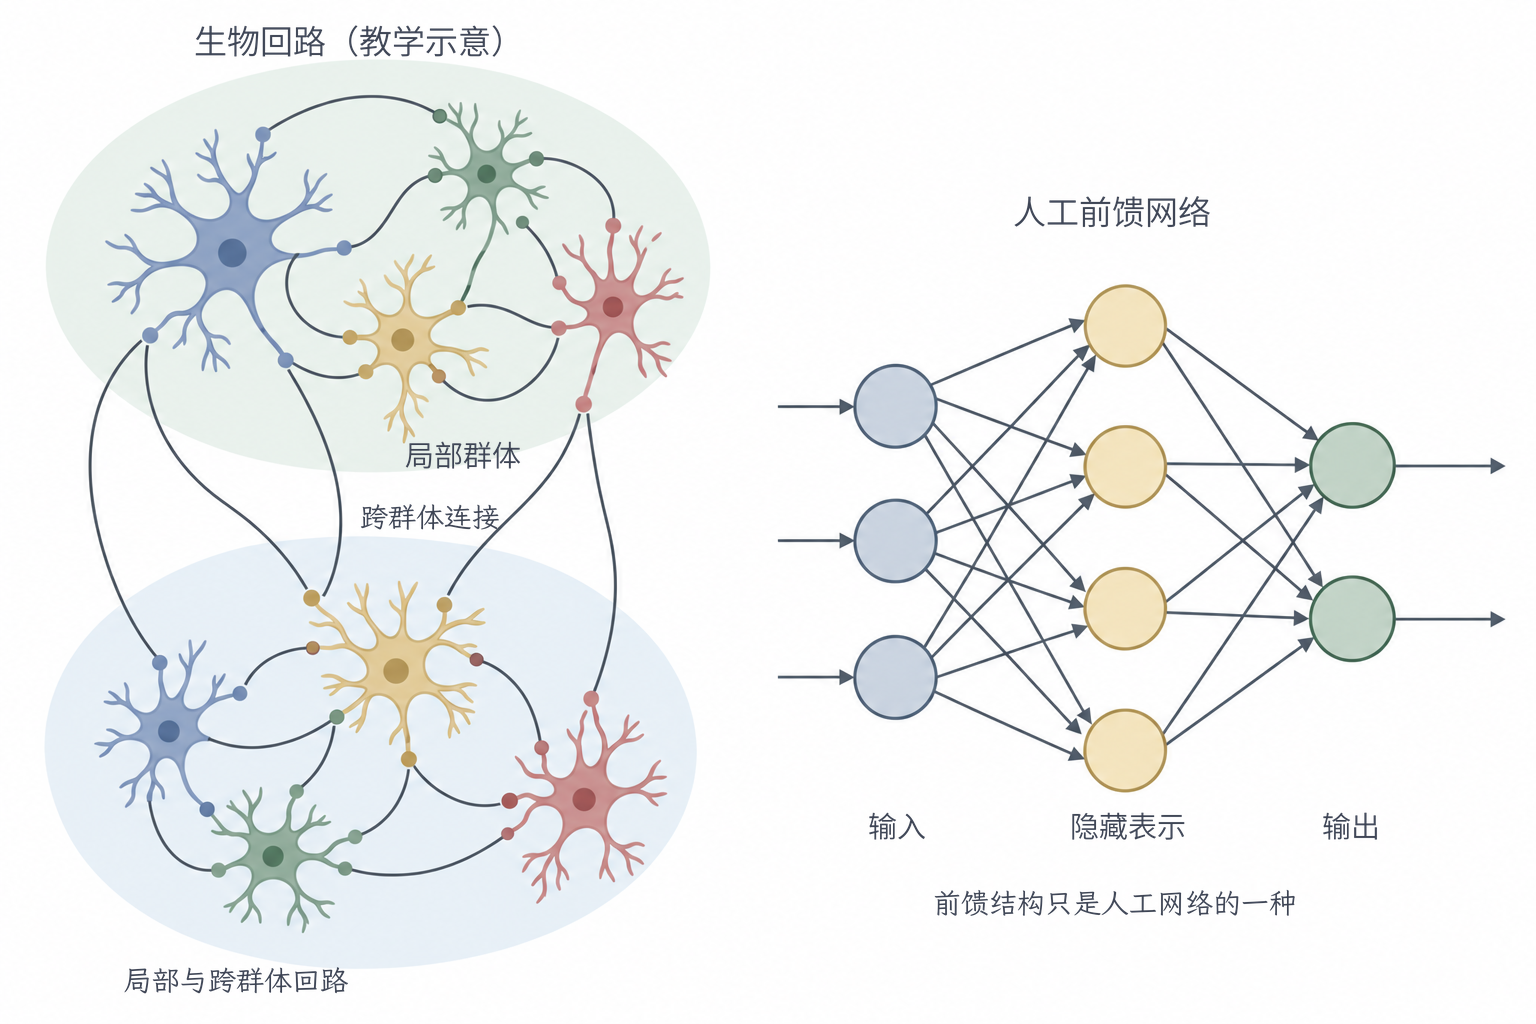
\includegraphics[width=130.048mm]{figures/05-neural-network-models/00-shared/generated/neural-biological-artificial-networks/figure.png}
  \caption{生物回路与前馈人工网络的组织示意。左侧表示细胞差异、局部群体及跨群体联系，是教学构造；右侧箭头表示输入、中间表示与输出的计算依赖。节点数量不表示真实规模，右图不涵盖所有人工结构。}
  \label{fig:neural-biological-artificial-networks}
\end{figure*}

视觉机制的生物学发现确实多次启发了人工结构。\term{新认知机}（neocognitron）交替组织局部模式检测与响应汇集，使识别对一定范围内的位置变化更容忍\scite{fukushima1980}卷积网络沿用局部连接与参数共享组织图像计算，其中参数共享更多是出于效率和统计考虑的工程约束，而非对生物事实的复刻；脉冲网络则选择保留“发放事件及其精确时间”这一维度（见本卷脉冲网络章）。它们分别借鉴了生物系统的不同侧面，没有一个试图复制全部机制。

在“学习”这一点上，两类系统的共同点是经验能够改变连接强度，更新依据却可以完全不同。标准的\term{误差反向传播}（error backpropagation）先完成一次前向计算，再利用整体任务损失对每个参数求梯度，让输出端的错误逐层传回每一条连接；赫布规则、STDP这类局部规则则只根据一个突触两端的活动决定变化，不直接知道整体行为的好坏。目前关于生物反馈通路和可塑性的研究，尚不能证明大脑执行的是标准反向传播；反过来，人工网络也不排斥使用局部学习规则\scite{lillicrap2020}。因此选择单元形式、连接方式、信号编码和学习规则时，应当服从模型要解释的现象或要完成的任务，而不以“是否更像大脑”为标准。

\section{神经网络的类型}
\label{sec:neural-network-types}

经过前面的讨论，我们已经可以凭直觉描述网络：输入经过若干层非线性变换得到输出，层间连接可以遵循各种结构假设。但打开任何一篇论文都会遇到一大堆名字：卷积网络、循环网络、图网络、Transformer、脉冲网络、注意力网络……新手常误以为它们是一张互斥清单上的并列选项。事实上，这些名字强调的是网络的不同侧面。本节给出三个相互独立的判断维度：计算依赖如何组织（\ref{sec:neural-types-connectivity}节）、信息以什么方式交互（\ref{sec:neural-types-interaction}节）、单元用什么形式的信号承载信息（\ref{sec:neural-types-encoding}节）。同一个具体网络通常可以在三个维度上分别被描述，三个维度的回答可以自由交叉；读完本节后应能回答：“卷积网络能不能是循环的？”“图网络和前馈网络矛盾吗？”这一类问题。

\subsection{按连接结构划分}
\label{sec:neural-types-connectivity}

这一维度考察的是\textbf{层或模块之间的连接是否形成有向回返}，即计算中是否存在一条从某单元出发、沿箭头又回到该单元的路径。

\term{前馈神经网络}（feedforward neural network）的层间依赖不包含任何有向环：信息从输入出发，沿依赖关系单向流向输出，每个单元只被计算一次。允许跨层的跳接（让某层直接读取更早层的输出），只要不构成回返，网络仍是前馈的。\term{循环神经网络}（recurrent neural network, RNN）则把前一次计算留下的内部状态用于下一次更新：当前输出不仅取决于当前输入，还取决于上一步保存下来的状态；由于状态在时间步之间反复读写，展开来看就形成了环。循环网络通常在多个时间步复用同一组更新参数。

用同一个句子分类任务可以看清差异。对“这部电影并不好看”这样的评论，前馈网络需要先把整句整理成一个定长向量，再一次性读取它作出判断；循环网络则逐词读入，读到“不”时状态发生改变，这个改变后的状态继续参与读到“好”“看”时的计算，于是否定关系有了一条自然的表达路径。需要特别注意两点区分依据：判断前馈还是循环，看的是\emph{状态是否在计算步骤之间传递}，而不是“输入是不是序列”——前馈网络也可以处理序列（只要序列被预先整理成定长表示）；也不是“参数是否共享”——共享参数本身不构成环。循环更新按时间展开后，每个时间步内部仍是按先后顺序的普通计算，所以它并不神秘，只是把同一个计算重复施加在“输入+此前状态”上。

树形和图形数据描述的是另一种结构特征，它们回答“输入对象本身有没有内部关系结构”，与有没有环是两回事。\term{树递归网络}（recursive neural network）按父子关系递归组合表示，例如把句子的短语结构分析成树，先组合子短语的表示，再由子短语形成整句表示。\term{图神经网络}（graph neural network, GNN）则直接利用输入中实体之间的关系，例如把路口网络建模为图，路口是节点、道路是边，每个节点的新表示由其道路相连的邻居聚合而成。关键在于：即使输入图本身带有环（城市道路中随处可见的环路），网络也可以规定“每一层只读取上一层留下的表示”，于是一次更新内部的信息流向仍然是前馈的。因此“图网络”并不是与“前馈、循环”并列互斥的第三类：它说的是计算沿输入给定的关系结构进行，而前馈/循环说的是这些计算依赖本身有没有回返。此外，\term{状态空间模型}（state space model, SSM）用一个连续的内部状态概括历史，再由状态读出输出，是循环思路的另一种常见数学形式。

图~\ref{fig:neural-topologies}分别展示无回返的前馈依赖、循环更新沿时间展开后的形态，以及按输入图读取邻居的一次聚合。任何网络最终都能画成一张由节点和箭头构成的计算图；“图神经网络”特指\emph{利用输入数据自带的关系结构}来组织表示的模型，而不是泛指所有“长得像图”的网络。
\begin{figure}[htbp]
  \centering
  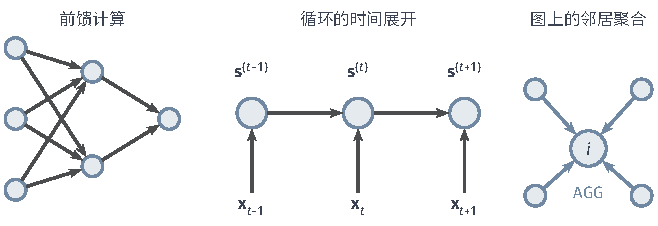
\includegraphics[width=111.361mm]{figures/05-neural-network-models/00-shared/tikz/neural-topologies/figure.pdf}
  \caption{三种结构视角。左侧为无回返的前馈依赖；中间为循环更新的时间展开，各步共享状态更新参数；右侧为图网络的一次邻居聚合，邻居向中心节点$i$提供信息。输入图的环不等于一次更新中的计算循环。}
  \label{fig:neural-topologies}
\end{figure}
\FloatBarrier

\subsection{按信息交互方式划分}
\label{sec:neural-types-interaction}

确定计算依赖的大框架后，下一个问题是：当一个单元要综合多个来源的信息时，它\textbf{能读取多大范围、来源关系由谁决定、各个来源的权重如何形成}？常见机制正是在这三点上不同；它们不是互斥类型，而常常出现在同一个网络的不同层中。

\term{全连接}（fully connected）让每个输出单元读取上一层的全部坐标，每条连接都有一个独立的、待学习的权重。\term{卷积}（convolution）通常作用于规则网格（如图像像素），每个单元只读取一个局部邻域，而且同一组权重在网格的所有位置复用。仍以边缘检测为例：一条竖直边缘无论出现在左上角还是右下角，在统计上是同一种局部模式，用同一组权重检测即可，无需为每个位置单独学一份。二者的差别可以归结为“一次读取的范围”和“权重是否跨位置共享”；它们都可以放在前馈网络中，一个卷积网络的末端也常接全连接层，因此“卷积还是全连接”是针对\emph{层}的提问，不是针对整个网络的非此即彼。

当输入的关系不规则时，读取范围可以直接由输入关系给出。\term{消息传递}（message passing）按输入图确定每个节点可以读取的来源——它的邻居——再把邻居发来的信息聚合起来；不同节点的邻居数量不必相同，正如每个路口相连的道路数不同。另一种机制改变的是权重的形成方式。\term{注意力机制}（attention mechanism）不让权重固定，而是根据当前表示，临时计算各信息来源在\emph{这一次}组合中应占的份额。用交通网络作比：消息传递回答“我听哪些路口”（由道路连接决定，固定不变），注意力回答“这次我更该听谁”（取决于当前路况，随内容变化）。同一个路口节点可以在按邻居聚合的同时，用注意力给各邻居分配动态权重，两种机制天然可以叠加。注意力的读取范围也不必是全体单元，可以限定在一个局部窗口或图邻居内，使用注意力并不意味着所有单元必须彼此相连。

注意力同样可以用于序列中各位置之间的交互，但允许读取哪些位置仍要根据任务规定：对一个完整句子作编码时，每个词都可以读取整句的上下文；而在逐步续写时，当前位置不能读取尚未生成的后续内容，否则等于偷看答案。还要区分两种“权重”：随每次输入变化的是注意力的组合系数（由当前内容临时算出），而网络中待训练的参数（决定“如何计算这些系数”的那些权重）是固定的、不会在一次预测中被重新训练。\term{Transformer}以注意力组织位置间交互，同时每个位置还配有独立的前馈变换；卷积或循环网络也可以在某些层插入注意力模块。因此判断一个模块的交互方式时，应直接考察该模块读取范围、关系来源和系数形成方式，而不能用整个架构的名字代替分析。

\subsection{按信息编码方式划分}
\label{sec:neural-types-encoding}

第三个维度考察的是\textbf{单元之间传递的信号本身}：是连续数值，还是离散的发放事件。

\term{连续值激活}（continuous-valued activation）用数值的大小承载信息：单元的输出是一个实数，数值越大通常表示响应越强，前面各节的网络都采用这种方式。这里的“连续值”是数学模型层面的描述；在计算机中任何数值都以有限精度存储，这不影响模型语义。

\term{脉冲神经网络}（spiking neural network, SNN）则模仿生物神经元，以离散的发放事件传递信息：单元在大部分时间沉默，只在特定时刻发出脉冲。信息可以编码在多个方面——一段时间内发放的脉冲数量（发放越密集表示响应越强）、脉冲发放的精确时刻，或多个单元脉冲之间的相对时序。这里需要区分对外信号与内部状态：单元向外发送的是离散脉冲，但它内部的膜电位等状态变量仍可取连续值并随时间连续演化；“脉冲网络是二值网络”是常见误解。

编码方式与前两个维度彼此独立：脉冲网络可以用卷积组织空间连接，可以是前馈的，也可以带循环连接；一个层间前馈的脉冲网络，单元内部仍可保留对历史的电位记忆。脉冲事件式的通信在生物学上更真实，在特定低功耗硬件上也可能因为“大部分单元大部分时间不活动”而节省能耗，但是否真的节能，还需结合活动密度、运行时间和具体实现条件综合评价，不能仅凭“脉冲”二字断定。

表~\ref{tab:neural-cross-classification}把三个维度的回答交叉起来。可以看到，一个带注意力的循环网络在连接组织上递推状态、在交互方式上按内容动态聚合、在编码上仍用连续值；而前馈脉冲卷积网络同时具备层间前馈、局部共享和脉冲事件三种性质。每一列回答的是不同问题，记住这一点，面对新架构名称时就知道该把它拆到哪些维度上理解。
\begin{table*}[htbp]
  \centering
  \small
  \begin{tabularx}{\linewidth}{@{}>{\RaggedRight\arraybackslash}p{45mm}>{\RaggedRight\arraybackslash}p{42mm}>{\RaggedRight\arraybackslash}X>{\RaggedRight\arraybackslash}p{26mm}@{}}
    \toprule
    \textbf{代表形式} & \textbf{连接组织} & \textbf{主要交互} & \textbf{信号编码} \\
    \midrule
    层状全连接网络 & 层间前馈 & 稠密加权组合 & 连续值激活 \\
    前馈卷积网络 & 层间前馈 & 局部连接与参数共享 & 连续值激活 \\
    带注意力的循环网络 & 状态递推 & 状态更新与动态聚合 & 连续值激活 \\
    固定轮数的图消息传递网络 & 按轮次展开 & 按输入图聚合邻居 & 连续值激活 \\
    前馈脉冲卷积网络 & 层间前馈，单元保留状态 & 局部连接与参数共享 & 脉冲事件 \\
    \bottomrule
  \end{tabularx}
  \caption{同一网络可以按连接组织、交互机制和信号编码分别描述。表中是展示交叉关系的代表形式，不穷尽同名网络的变体。}
  \label{tab:neural-cross-classification}
\end{table*}

\FloatBarrier

\section{神经网络的历史}
\label{sec:neural-history}

神经网络常给人“突然爆发”的印象，但它的主要思想是在几十年里围绕三个相互联系的问题逐步展开的：第一，怎样用相互连接的简单单元\emph{表达}计算（结构问题）；第二，连接中的参数怎样从经验中\emph{获得}（学习问题）；第三，在有限的数据和计算条件下怎样\emph{用得起}这些网络（规模问题）。历史中的代表性工作，分别在这三个环节上移除了一个具体障碍。图\ref{fig:neural-network-history}与图\ref{fig:neural-network-history-recent}按时间展示代表工作，年份采用论文发表或首次公开时间。阅读时请保持两个意识：这些机制解决的是不同环节的问题，因而大多可以组合使用，时间先后不表示“后者淘汰前者”；许多思想都经历过早于流行年份的铺垫，本节标注的是形成广泛影响的代表工作。

% 历史图分别随早期与近期机制说明排布，保留可读字号并为相关正文留出空间。
\Needspace{10\baselineskip}
\subsection{从阈值单元到可学习网络}
\label{sec:neural-history-threshold}

最早的问题是：相互连接的简单单元，原则上能完成什么计算？1943年，McCulloch和Pitts给出了一种理想化的二值神经元：每个单元对若干二值输入加权求和，再与固定阈值比较，决定输出$0$或$1$；通过合适地安排连接，网络可以实现各种逻辑组合。这个模型的意义在于第一次形式化地说明“神经元式的网络可以执行逻辑计算”，但它的权重和阈值全部由设计者手工指定，网络本身并不学习，因此它还不是现代意义上的机器学习模型\scite{mcculloch1943}

如果权重能够随经验改变，网络就有机会自己从样本中归纳分类规则。Rosenblatt在1958年提出的感知机（perceptron）把这一步走了出来：基础形式对输入加权后按阈值输出类别，并在每次预测错误后，按错误方向小幅调整相应权重——把判错的正样本相关权重调高、判错的负样本相关权重调低，规则简单到可以用电硬件实现，在当时引起轰动。需要说明，Rosenblatt的原始体系包含感觉单元、联想单元和反应单元等更丰富的组织，不应把其中所有形式都等同于今天教科书里的单层线性分类器\scite{rosenblatt1958}

热情随后遇到了能力边界。Minsky和Papert在1969年分析指出，没有隐藏层的感知机只能学习线性可分的函数，示例~\ref{ex:neural-xor-representation}中的异或就是它无法解决的最简单反例。这个批评的实质不是“神经元式计算行不通”，而是指出了单层的局限；而当时虽然知道加入隐藏单元可以扩大可表达函数的范围（异或例子已证明这一点），却没有一个被广泛认可的、能决定隐藏层权重的训练算法——隐藏单元没有自己的标签，谁来告诉它们该学什么？这个信用分配难题使神经网络研究进入了一段相对低潮，直到有效的多层训练方法出现。

\begin{figure*}[!t]
  \centering
  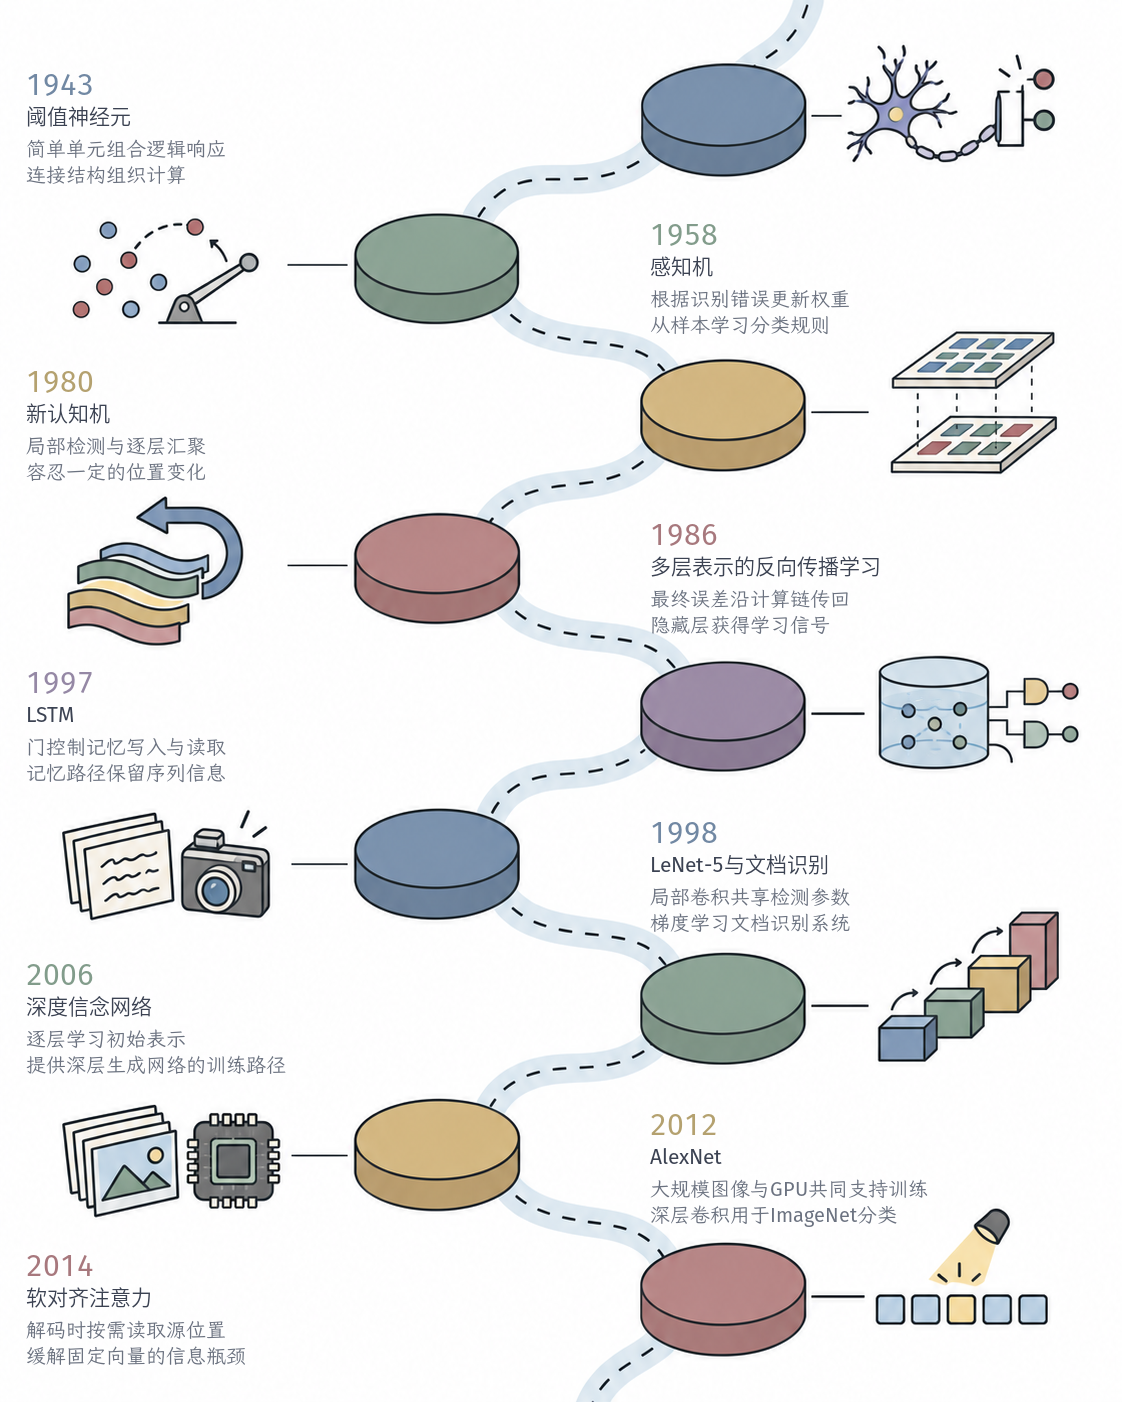
\includegraphics[width=149mm]{figures/05-neural-network-models/00-shared/generated/neural-network-history/figure.png}
  \caption{神经网络发展的代表工作（1943—2014）。沿虚线路线从上向下阅读，文字指出各项工作改变的计算或学习机制。年份采用代表论文的首次公开或发表时间；节点间距不按时间比例绘制，先后不表示替代。}
  \label{fig:neural-network-history}
\end{figure*}

\subsection{从浅层学习到深层训练}
\label{sec:neural-history-deep-training}

要让隐藏层参与学习，输出端的错误必须能转化为对每个内部参数的调整量。微积分其实已经提供了工具：复合函数可以用链式法则逐层求导。1986年，Rumelhart、Hinton和Williams系统展示了用误差反向传播训练多层网络的方法——先前向计算预测和损失，再沿计算的反方向逐层求出损失对每个参数的偏导，配合梯度下降更新。这使“没有标签的内部单元”第一次有了明确的学习信号：它的梯度由它对后续层、最终对损失的贡献决定。反向传播成为多层表示学习的代表性起点，但链式求导本身是已有数学工具，相关思想在不同领域也有更早的探索，不应把1986年当作一切相关算法的统一起点\scite{rumelhart1986}

学习规则之外，结构可以直接利用任务中的先验规律。1980年的新认知机已经用局部特征检测和逐层汇聚研究位置变化下的识别，不过它采用的是自组织式学习，不同于后来的监督梯度训练\scite{fukushima1980}卷积网络把局部连接、参数共享与反向传播结合：同一种局部模式检测在所有位置复用，既大幅减少参数，又契合图像统计规律。LeCun等人1998年用于手写文档识别的LeNet，展示了这种结构与基于梯度的整体训练结合后的实际效果\scite{lecun1998}

序列任务提出了另一个问题：如何让很久以前的输入影响当前输出？普通循环网络在时间维度上反复应用同一函数，相当于一个很深的复合结构，反向传播时梯度在连乘中容易逐层衰减或放大，远处信息的影响和它对应的学习信号都可能消失。Hochreiter和Schmidhuber在1997年提出的\term{长短期记忆}（long short-term memory, LSTM），为信息增设了一条受门控的“记忆通道”：输入门、遗忘门和输出门这些可学习的开关决定哪些新信息写入、哪些旧信息保留、哪些内容读出，使网络有可能跨越很多时间步维持信息。它为长期依赖提供了更合适的计算路径，但门控只是\emph{允许}信息长期保存，实际能学到多长的依赖仍取决于训练设置和数据\scite{hochreiter1997}

在反向传播已可用之后，深网络一度仍然难训，逐层预训练提供了一条过渡路径。2006年的\term{深度信念网络}（deep belief network, DBN）用多层潜变量描述数据的生成过程，即建模“可能观测到的数据”的概率分布；训练时先无监督地学好一层，再把这层的表示当作下一层的输入继续学习，逐层堆叠后再整体微调。它证明了深层结构是可以训练的，并推动了深度生成模型的发展，但这条路线不同于直接按分类损失端到端训练所有层\scite{hinton2006deepbelief}

真正让深层网络在主流任务上展现压倒性效果的，是数据、计算与结构三者的汇合。2012年的AlexNet在ImageNet大规模图像分类竞赛中大幅领先传统方法：它依赖上百万张带标注图像、用图形处理器（graphics processing unit, GPU）承担原本难以负担的并行训练计算，并配合了ReLU激活、 dropout正则化等结构与训练设计。这项成果说明的是配合效应，而不是“层数越多越准”的简单结论\scite{krizhevsky2012}。网络继续加深后又出现新的优化困难：层数过多时，梯度路径过长，训练误差反而可能上升。\term{残差连接}（residual connection）给出的办法是，在维度相容时让输入通过一条“直达通路”与若干层变换的结果相加：$\bm{x}_{\text{out}}=\bm{x}+F(\bm{x})$，于是中间层只需学习“在已有表示上还要补充的变化”$F$，梯度也可以沿直达通路传回。残差网络使训练上百层的网络成为可能；卷积、门控记忆和残差连接改变的是不同环节，因此可以在同一模型中配合使用\scite{he2016resnet}

\subsection{从固定连接到内容相关计算}
\label{sec:neural-history-content-dependent}

前述网络无论深浅，一个单元读取哪些来源、以多大权重组合，在训练完成后就固定下来（输入内容只改变被送来的数值）。序列任务暴露了这种固定方式的局限：一次预测往往只需要历史中的一小部分，而把整段输入不分轻重地压进一个定长向量，信息可能在压缩中丢失。

机器翻译是典型例子：生成译文的每个词时，真正需要对齐的常常只是原句中的某几个词。Bahdanau、Cho和Bengio在2014年公开、2015年正式发表的研究中提出，让解码器在生成每个译词时，根据当前解码状态临时计算对原句各位置表示的权重，再加权组合出“此刻该看的原文信息”。注意力与循环网络的这次结合，改变的是\emph{每次计算读取信息的方式}，读取权重随内容动态生成\scite{bahdanau2015}

2017年的Transformer把注意力从循环结构的配角提升为组织计算的核心：用\term{自注意力}（self-attention）让同一组输入中的各个位置根据彼此的内容直接交换信息，再配合每个位置上独立的前馈变换逐层加工。由于一次自注意力中所有位置的读取都只依赖该层入口已有的表示，它们可以并行计算，摆脱了循环网络必须按时间步串行的限制。需要补充的是，这种并行性适用于输入完整给定的情形；在自回归生成时每个新位置只能看到此前的内容，整段输出无法同时产生\scite{vaswani2017}

内容还可以决定“本次由哪些计算单元参与”。\term{混合专家}（mixture of experts, MoE）准备多个有所分工的子网络（即“专家”），再由一个路由网络根据当前输入决定激活、组合其中哪几个。Shazeer等人2017年的稀疏门控工作让每个输入只启用一小部分专家，从而把“模型总共存储了多少参数”与“单次预测实际计算多少参数”分开：总容量可以很大，单例成本却较小。当然，路由判断本身、把数据分配到不同设备以及汇集结果都会带来额外开销，实际收益要计入这些成本\scite{shazeer2017}

另一条路线保留“状态递推”的视角，专门改进长序列处理：状态负责把此前所有输入的影响浓缩传递，每一步由状态更新和读出完成计算。2021年公开、2022年发表的\term{结构化状态空间序列模型}（structured state space sequence model, S4）用一种特殊结构的状态矩阵组织递推，在特定条件下把状态递推与卷积计算联系起来，使训练稳定性和长程依赖都得到改善\scite{gu2022s4}；2023年的Mamba进一步让状态更新中的部分系数随当前输入变化，从而有选择地保留或遗忘信息\scite{gu2023mamba}。这些方法与注意力分别从“递推压缩”和“直接检索”两个方向组织信息读取。它们也提醒读者注意三类量的区别：训练后固定保存的模型参数、随每次输入变化的注意力权重或专家路由、以及随时间步演化的递推状态。

\begin{figure*}[!t]
  \centering
  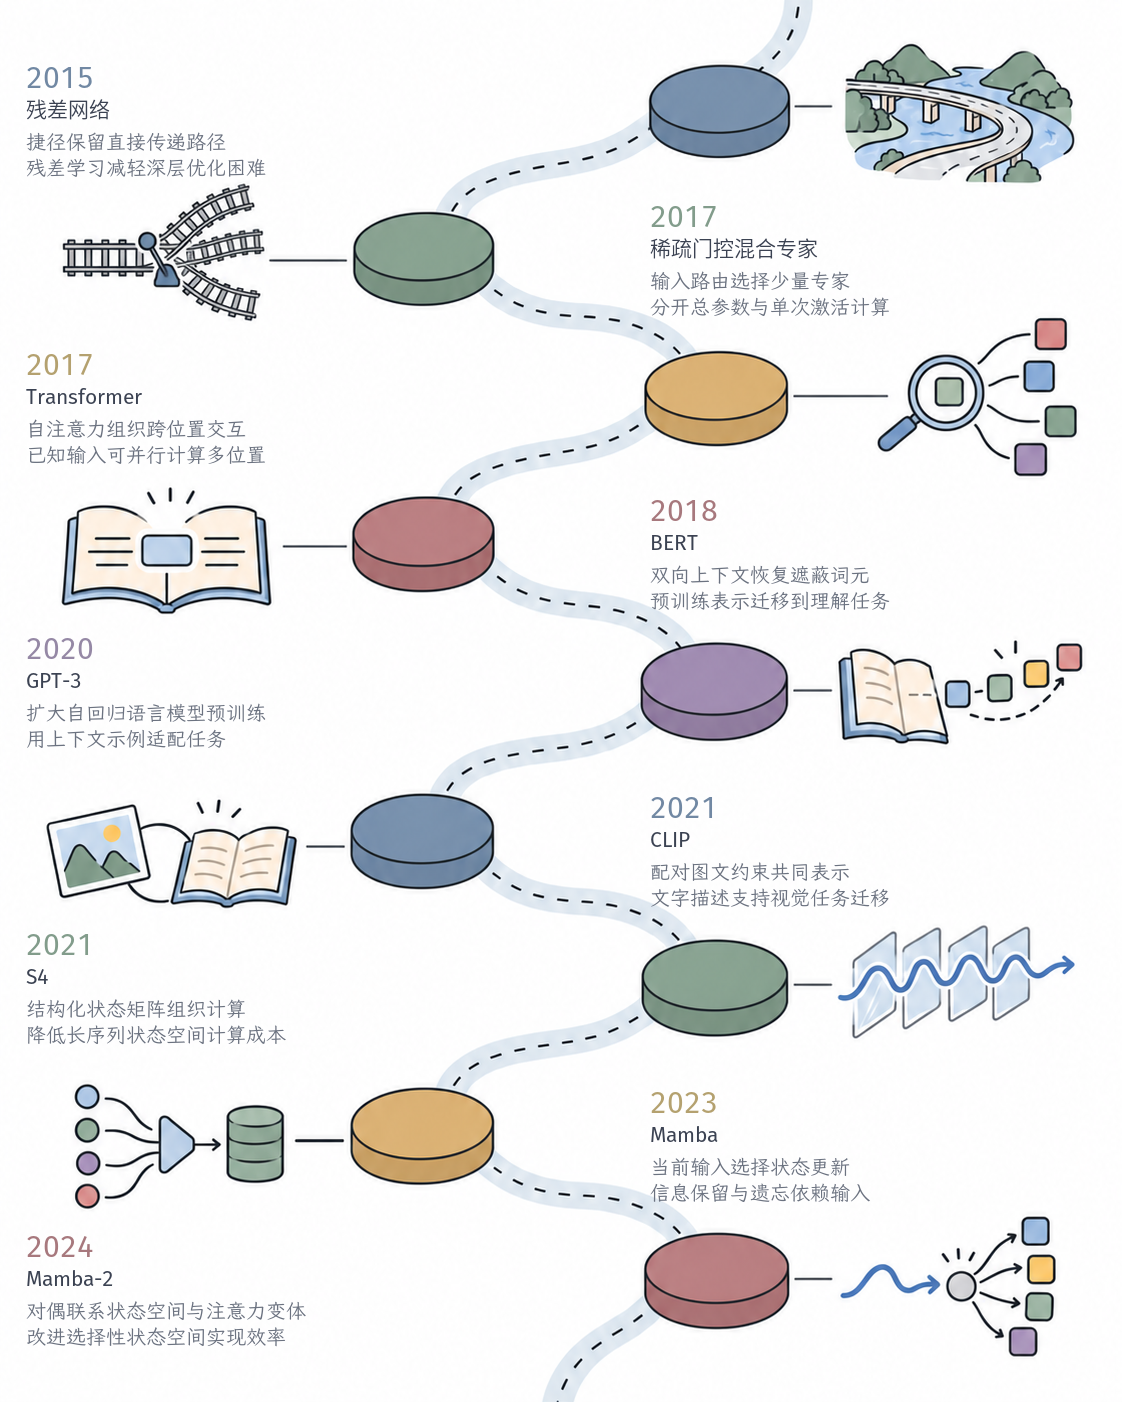
\includegraphics[width=149mm]{figures/05-neural-network-models/00-shared/generated/neural-network-history-recent/figure.png}
  \caption{神经网络发展的代表工作（2015—2024），承接图\ref{fig:neural-network-history}。各节点分别改变深层路径、内容读取、训练信息或资源组织，相应机制可以组合使用。读法和日期口径与前图相同。}
  \label{fig:neural-network-history-recent}
\end{figure*}

\subsection{面向能力、成本与可靠性的探索}
\label{sec:neural-history-current}

监督学习依赖大量人工标签，而现实中绝大多数观测没有标签，却并非不含信息。\term{自监督学习}（self-supervised learning）从数据本身构造训练目标：把输入的一部分遮住或挪走，让模型利用剩余部分预测被隐藏的内容，这样无须人工标注，原始记录自身就提供了答案。\term{预训练}（pre-training）是与之配合的训练安排：先在大规模数据上学习通用参数或表示，再把这些参数用于具体任务；它本身不指定目标，自监督、监督都可用于预训练。代表性工作中，BERT利用一个词左右两侧的上下文恢复被遮住的文本单位，GPT系列则按已有前缀逐步预测后续文本；GPT-3还研究了在不更新参数的情况下，用当前输入里给出的任务示例引导模型处理新任务的用法\scite{devlin2019,brown2020}。当信息来自不止一种模态时，\term{多模态学习}（multimodal learning）联合利用如图像与文本等不同类型的数据，CLIP用大量配对的图文学习把两者映射到同一表示空间，使文字描述可以直接参与视觉任务的定义\scite{radford2021}。这些方法扩大了模型可利用的信息来源，但是否能迁移到新任务，仍取决于预训练数据的覆盖面与目标任务的差距。

规模扩大同时带来现实的计算与存储约束。2024年前后的代表性工作继续在“能力—成本”之间寻找空间：Mamba-2利用特定条件下状态空间模型与一类注意力计算之间的数学联系改进计算组织；DeepSeek-V3继续研究稀疏专家架构下的训练与执行安排\scite{dao2024mamba2,deepseek2024v3}。增加总参数量、减少单次激活的专家数、压缩需要保存的历史状态，针对的是不同的资源账单：状态压缩可能丢掉任务真正需要的远期信息，稀疏专家仍需在设备间路由和汇集结果，因此任何效率结论都要结合任务规模与硬件实现评价，不能只比较参数总数。

最后，能力评价正在与可靠性评价分开。基准测试上的高正确率，并不能单独回答这些同样重要的问题：模型给出的概率是否可信地反映不确定性？换到来源不同的数据上是否仍然有效？生成的陈述是否符合事实？改进手段也应区分两类：后训练通过进一步学习实际改变模型参数（如针对人类偏好的调整）；推理阶段的技术则不改动参数，而是在本次预测中增加候选生成、搜索或验证步骤。两者都可能提高某项指标，也都带来额外计算成本。面对任何新工作，只有先明确它的任务定义、数据范围和检验对象，才能判断它究竟移除了哪个环节的障碍。

\FloatBarrier

\section{本章小结}
\label{sec:neural-overview-summary}

本章围绕“神经网络比传统线性模型多了什么”展开。核心答案是：神经网络把\emph{表示变换}纳入学习范围——隐藏层在任务损失的引导下改造输入坐标，使后续层在更友好的表示上完成预测；非线性激活是多层网络区别于单层线性模型的关键，没有它，任意多层线性变换都会合并成一次线性变换。同层内多个单元分布式地共同表示信息，不同层之间层次化地逐级组合更复杂的特征；网络结构则通过局部连接、参数共享、隐状态等设计注入归纳偏置，在利用数据规律的同时也限定了可表达的函数。表示能力、优化和泛化是三个必须分开评价的问题。

人工神经网络从生物神经系统借用了名称和功能直觉：人工单元对应“多输入整合后决定输出”，但舍去了脉冲时序、化学突触和动态膜电位；结构上的局部处理与层次组合受视觉系统启发，学习规则上则与赫布可塑性等局部机制分道扬镳，标准反向传播依据的是整体任务损失。判断一个网络应分别考察三个相互独立的维度：层间连接是否有回返（前馈还是循环）、信息按什么范围和权重交互（全连接、卷积、消息传递、注意力）、信号用连续值还是脉冲事件编码；这些描述可以自由交叉。

历史回顾则显示，这个领域围绕相继出现的障碍推进：阈值单元回答“网络能计算什么”，感知机把权重变为可学习，异或批评暴露了单层局限，反向传播解决了隐藏层的信用分配，卷积、LSTM、残差连接等结构分别利用了图像、序列和深度上的规律，注意力、专家路由和状态空间模型让计算随内容或历史组织，自监督预训练与多模态学习扩展了训练信息的来源，而成本与可靠性成为当前与能力并列的评价对象。后续章节将依次介绍前馈、卷积、循环、图、注意力与脉冲等具体架构，以及训练与泛化的系统方法；读者可以带着“它改变了三个问题中的哪一个”这一视角进入后续内容。

\paragraph{扩展阅读}
Goodfellow等的《深度学习》系统介绍表示、优化与统计学习，Bishop与Bishop的教材进一步联系现代网络结构\scite{goodfellow2016,bishop2024deep}
